\documentclass[14pt, a4paper]{extarticle}	
\usepackage{GOST}

\makeatletter
\renewcommand\@biblabel[1]{#1.}
\makeatother


\graphicspath{{images/}}

\begin{document}
\setcounter{page}{3}

% СОДЕРЖАНИЕ 
\clearpage
\tableofcontents

\clearpage
\section*{Введение}
\addcontentsline{toc}{section}{Введение}
	Современные вычислительные системы сложно представить без поддержки интернет-сетей. На одном устройстве может быть доступ к различным подсетям по различным сетевым интерфесам и каналам передачи данных. Однако, со стороны пользовательского программного обеспечения может быть неудобно обращаться к различным сетевым интерфейсам. Агрегация нескольких сетевых интерфейсов в один может облегчить доступ к нескольким подсетям со стороны прикладных приложений.\\
\indent Так как сетевой интерфейс может быть определен в системе только с помощью загружаемого модуля ядра, то данная работа будет основана на анализе и разработки такого загружаемого модуля.


\clearpage
\section{Аналитический раздел}
\subsection{Постановка задачи}
В соответствии с заданием на курсовую работу необходимо разработать
и реализовать загружаемый модуль ядра, реализующий создание виртуального интерфейса для распределения пакетов по уже существующим сетевым интерфейсам. \\
\indent Для достижения цели курсовой работы необходимо решить следующие задачи:
\begin{itemize}
	\item проанализировать пути решения задачи;
	\item спроектировать модуль, реализующий необходимую функциональность;
	\item реализовать спроектированный модуль;
	\item протестировать реализованный модуль.
\end{itemize}
\indent Разрабатываемое ПО должно перенаправлять пакеты, пришедшие на виртуальный интерфейс по указанным интерфейсам в зависимости от IP назначения пакета.



\subsection{Загружаемый модуль ядра Linux}
Существует только один способов реализации требуемой функциональности --- загружаемый модуль ядра. \\
\indent Загружаемый модуль ядра --- модули, позволяющие расширять и модифицировать ядро операционной системы его перекомпиляции. Из модуля ядра могут напрямую вызыватся системные функции. Модуль ядра может реализовывать драйвер устройства, файловую систему и выполняется на нулевом кольце защиты, имеющим максимальный уровень привилегий [1].

\subsection{Сетевые интерфейсы и устройства}
Для доступа к сетевым устройствам используются так называемые сетевые интерфейсы. Лги являются основной сетевой подсистемы Linux. Все сетевое взаимодействие в Linux происходит через сетевые интерфейсы. Любые данные, которые компьютер отправляет в сеть или получает из сети проходят через сетевой интерфейс. \\
\indent Некоторые источники [2, 3] выделяют сетевые устройства в третий основной класс устройств в Linux, наравне с символьными и блочными. \\
\indent Однако интерфейсы это не файлы устройств и их нет в каталоге /dev. Интерфейсы создаются динамически и не всегда связаны с сетевыми картами. Например интерфейс ppp0 - это интерфейс VPNа, организованного по протоколу PPTP, а интерфейс lo это виртуальная сетевая карта с адресом localhost (127.0.0.1). Такие интерфейсы называются виртуальными. \\
\indent Таким образом сетевые интерфейсы скрывают детали реализации конкретного сетевого устройства, прикладное программное обеспечение, обращаясь к сетевому интерфейсу не учитывает детали реализации конкретных сетевых устройств. Однако в Linux существует общепринятая схема именования сетевых интерфейсов, состоящая из префикса типа сетевого устройства и заканчивающаяся номером иакого устройства. Примеры наименования интерфейсов:
\begin{itemize}
	\item eth0 --- первый сетевой интерфейс к карте Ethernet или картам WaveLan (Radio Ethernet);
	\item wlan0 --- сетевой интерфейс wi-fi адаптера;
	\item  lo --- сетевой интерфейс к виртуальной сетевой карте с адресом localhost (127.0.0.1);
	\item  eth1n3 --- четвертый сетевой  интерфейс второй группы к карте Ethernet или картам WaveLan (Radio Ethernet).
\end{itemize}
Интерфейсы создаются автоматически для каждого обнаруженного сетевого устройства при загрузке ядра ОС. \\
\indent Каждый интерфейс характеризуется определёнными параметрами, необходимыми для обеспечения его нормального функционирования, и в частности для сетевого обмена данными с помощью стека TCP/IP. Некоторые параметры интерфейса:
\begin{enumerate}
	\item IP-адрес;
	\item маска подсети;
	\item аппаратный адрес сетевого устройства, соответствующего интерфейсу.
	\item  eth1n3 --- четвертый сетевой  интерфейс второй группы к карте Ethernet или картам WaveLan (Radio Ethernet);
\end{enumerate}

И сетевой интерфейс и драйвер сетевого устройства описываются большой структурой ядра `net\_device`, о которой сами разработчики, из-за смешения в ней разных уровней абстракции, отзываются как о "большой ошибке", в коде ядра есть комментарий: "Actually, this whole structure is a big mistake".



\subsection{net\_device}
Основной структурой, которую использует сетевая подсистема Linux является struct net\_device (определена в <linux/netdevice.h>). Сама структура является слишком большой для полного приведения, поэтому рассмотрим только некоторые поля.
\begin{itemize}
\item char name[IFNAMSIZ] --- имя устройста;

\item unsigned long rmem\_end , unsigned long rmem\_start , unsigned long mem\_end , unsigned long mem\_start --- информация о памяти устройства. Данные поля содержат начало и конец разделяемой памяти устройства. Поля rmem служат для определения памяти для получения данных, а mem --- для передачи. По соглашению поля end устанавливаются, поэтому end - start = общему количеству доступной памяти на устройстве;

\item unsigned long base\_addr --- базовый адрес ввода-вывода сетевого интерфейса. Это поле, как и предыдущие, назначаются во время обнаружения устройства. Команда ifconfig может быть использована для отображения и модификации текущего значения;

\item unsigned char irq --- назначеный номер прерывания;

\item unsigned char if\_port --- показывает, какой порт используется в устройствах с несколькими портами, например устройства с поддержкой как коаксиального (IF\_PORT\_10BASE2) Ethernet соединения, так и Ethernet соединения с помощью витой пары (IF\_PORT\_10BASET). Полный список известных типов портов определен в <linux/netdevice.h>;

\item unsigned long state --- состояние устройства. Это поле включает несколько флагов. Драйвер обычно не использует эти флаги напрямую, но с помощью специальных функций;

\item void *priv --- указатель, зарезервированный для пользовательских данных;

\item struct net\_device *next --- указатель на следующее сетевое устройство в глобальном связанном списке сетевых устройств.

\end{itemize}

Большую часть информации, связанной с сетевыми интерфесами в структуре net\_device заполняют существующие функции установки, определенные в <drivers/net/net\_init.c>. Примеры таких функций:
\begin{enumerate}
	\item void ether\_setup(struct net\_device *dev) --- инициализирует поля для устройств Ethernet;
	\item void ltalk\_setup(struct net\_device *dev) --- инициализирует поля для устройств LocalTalk;
	\item void fc\_setup(struct net\_device *dev) --- инициализирует поля для волоконно-оптических устройств;
	\item void fddi\_setup(struct net\_device *dev) --- конфигурирует интерфейс для сети с Fiber Distributed Data Interface (распределенным интерфейсом передачи данных по волоконно-оптическим каналам, FDDI).
	\item void hippi\_setup(struct net\_device *dev) --- инициализирует поля для High-Performance Parallel Interface (высокопроизводительного параллельного интерфейса, HIPPI);
	\item void tr\_setup(struct net\_device *dev) --- выполняет настройку для сетевых интерфейсов token ring (маркерное кольцо).
\end{enumerate}
Большинство устройств подходит под один из этих типов. Если требуется что-то уникальное, то необходимо определить следующие поля:
\begin{enumerate}
	\item unsigned short hard\_header\_len --- длина аппаратного заголовка;
	\item unsigned mtu - MTU (Max transfer unit);
	\item unsigned long tx\_queue\_len --- максимальная длина очереди на отправку;
	\item unsigned short type --- аппаратный тип интерфейса;
	\item unsigned char addr\_len --- длина аппаратного адреса;
	\item unsigned char dev\_addr[MAX\_ADDR\_LEN] --- аппаратный адрес устройства (MAC).
	\item unsigned short flags --- флаги интерфейса;
	\item int features --- специальные аппаратные возможности.
\end{enumerate}
Функции, с помощью которых система взаимодействует с устройством определены в структуре net\_device\_ops, определенной в <linux/netdevice.c>/ Часть структуры приведена ниже:
\begin{lstlisting}[caption=net\_device\_ops]
struct net_device_ops {
        int (*ndo_init)(struct net_device *dev);
        void (*ndo_uninit)(struct net_device *dev);
        int (*ndo_open)(struct net_device *dev);
        int (*ndo_stop)(struct net_device *dev);
        netdev_tx_t (*ndo_start_xmit) (struct sk_buff *skb, struct net_device *dev);
        void (*ndo_change_rx_flags)(struct net_device *dev, int flags);
        void (*ndo_set_rx_mode)(struct net_device *dev);
        void (*ndo_set_multicast_list)(struct net_device *dev);
        int (*ndo_set_mac_address)(struct net_device *dev, void *addr);
        int (*ndo_validate_addr)(struct net_device *dev);
        int (*ndo_set_config)(struct net_device *dev, struct ifmap *map);
        int (*ndo_change_mtu)(struct net_device *dev, int new_mtu);
        void (*ndo_tx_timeout) (struct net_device *dev);
        struct net_device_stats* (*ndo_get_stats)(struct net_device *dev);
        /* Several lines omitted */
};
\end{lstlisting}
Из них минимально необходимы:
\begin{enumerate}
	\item ndo\_open --- вызывается при открытии интерфейса;
	\item ndo\_close --- вызывается при закрытии интерфейса;
	\item ndo\_start\_xmit --- вызывается при передачи пакета через интерфейс.
\end{enumerate}




\subsection{Виртуальные интерфейсы tun/tap}
TUN и TAP — виртуальные сетевые драйверы ядра системы. Они представляют собой программные сетевые устройства, которые отличаются от обычных аппаратных сетевых карт. \\
\indent TAP эмулирует Ethernet устройство и работает на канальном уровне модели OSI, оперируя кадрами Ethernet. TUN (сетевой туннель) работает на сетевом уровне модели OSI, оперируя IP пакетами. TAP используется для создания сетевого моста, тогда как TUN для маршрутизации. \\
\indent Пакет, посылаемый операционной системой через TUN/TAP устройство обрабатывается программой, которая контролирует это устройство. Получение данных происходит через специальный файловый дескриптор, таким образом программа просто считывает данные с файлового дескриптора. Сама программа также может отправлять пакеты через TUN/TAP устройство выполняя запись в тот же файловый дескриптор. В таком случае TUN/TAP устройство доставляет (или «внедряет») такой пакет в сетевой стек операционной системы, эмулируя тем самым доставку пакета с внешнего устройства. \\
\indent Не смотря на внешнюю схожесть TAP интерфейса с планируемым решением, нельзя просто строить решение на его основе из-за различной внутренней логики виртуальных интерфейсов.



\subsection{Обработка пакетов на уровне сетевого интерфейса}
В сетевых интерфейсах существует очередь обрабатываемых пакетов.  На программном уровне следующий пакет из буфера пакетов, требующих обработки представлен структурой sk\_buff. \\
\indent На рисунке \ref{rx} проиллюстрирован процесс получения интернет-пакетов. Сетевые интерфейсы работают с пакетами 2-го и 3-го уровня модели OSI. Для применения к поставленной задачи необходимо как отправлять на несколько интерфейсов, так и считывать пакеты, отправленные в ответ. Для этого, как видно из схемы, необходимо вклинится в процесс обработки пакета. Linux позволяет добавить обработчик входящих пакетов с помощью функции netdev\_rx\_handler\_register.
\begin{figure}[H]
	\centering
	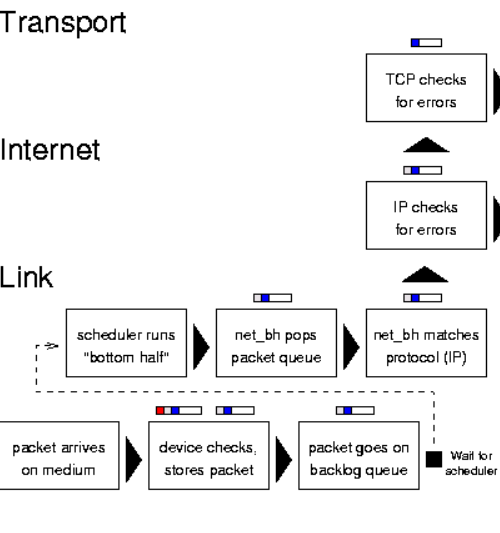
\includegraphics[scale=0.9]{r_rx.png}
	\caption{Обработка входящего пакета}
	\label{rx}
\end{figure}
\indent \indent Исходящий же пакет можно перенаправить на обработку в другой интерфейс с помощью подмены поля dev в структуре sk\_buff.
\clearpage
\section{Конструкторский раздел}
\subsection{Требования к программному обеспечению}
Программное обеспечение состоит из виртуального сетевого, реализованного в виде
загружаемого модуля ядра, который распределяет приходящие на него пакеты по существующим сетевым устройствам.

\subsection{Проектирование загружаемого модуля}
Общая структура загружаемого модуля представлена схемой на рисунке \ref{gen}.
\begin{figure}[H]
	\centering
	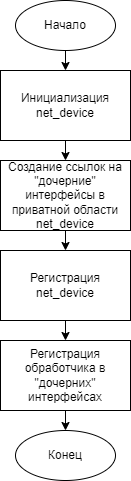
\includegraphics[scale=0.9]{gen.png}
	\caption{Общая структура загружаемого модуля}
	\label{gen}
\end{figure}

Схема алгоритма обработки принимаемого пакета на одном из интерфейсов, скрываемых виртуальным представлена на рисунке \ref{in}.
\begin{figure}[H]
	\centering
	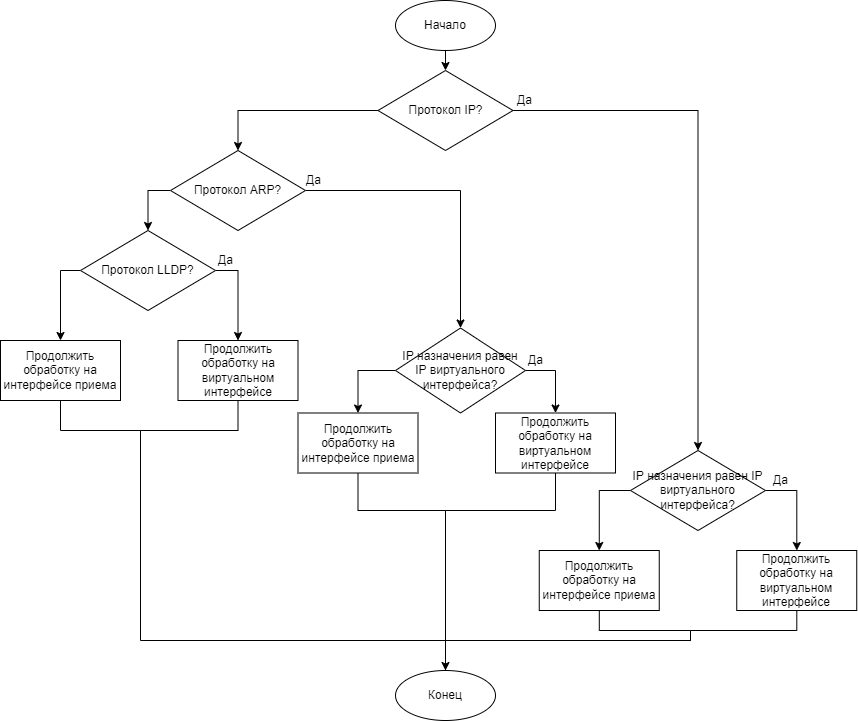
\includegraphics[scale=0.5]{in.png}
	\caption{Схема алгоритма обработки принимаемого пакета}
	\label{in}
\end{figure}

Схема алгоритма обработки отправляемого пакета, поступившего на виртуальный интерфейс представлена на рисунке \ref{out}.
\begin{figure}[H]
	\centering
	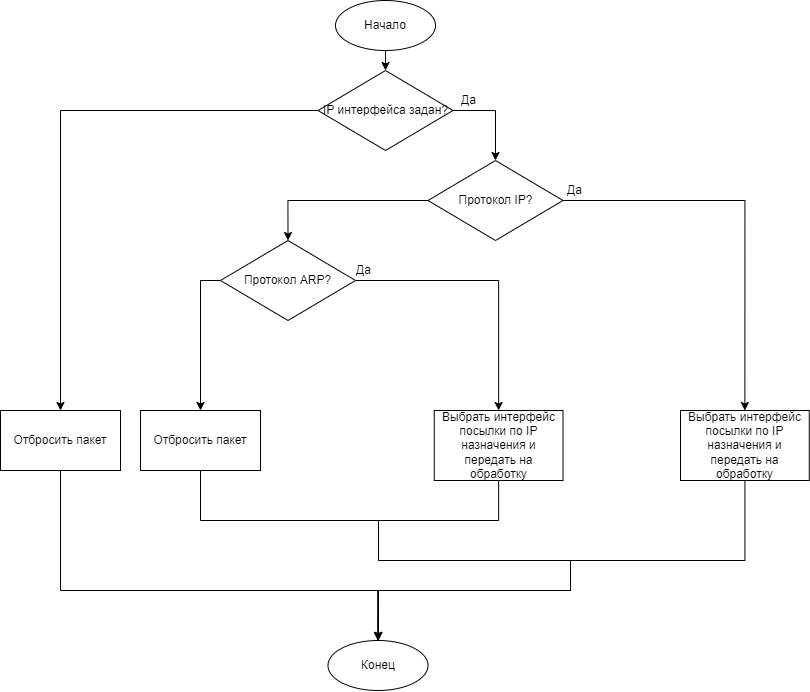
\includegraphics[scale=0.6]{out.png}
	\caption{Схема алгоритма обработки отправляемого пакета}
	\label{out}
\end{figure}

\clearpage
\section{Технологический раздел}
\subsection{Выбор языка программирования и среды программирования}
В качестве языка программирования для реализации поставленной
задачи был выбран язык С. Он является языком реализации модулей ядра и самого ядра ОС Linux. В качестве компилятора был использован
компилятор gcc. Средой разработки был выбран текстовый редактор Visual Studio Code.

\subsection{Описание реализации}
Для реализации хранения нескольких интерфейсов для распределения пакетов было принято решение хранить в связанном списке ссылки на структуры net\_device и дополнительную информацию об этих интерфейсах. Голова связанного списка хранится в приватной зоне памяти создаваемого виртуального интерфейса. На листинге \ref{linkd} Приведена структура узла вышеупомянутого связанного списка.

\begin{lstlisting}[caption=lst example, label={linkd}]
struct interfaces {
    u32 address; // адрес подсети
    u32 mask;    // маска подсети
    struct net_device *device; // ссылка на интерфейс
    struct interfaces *next;   // следующий узел
};
\end{lstlisting}

Для поиска подходящего интерфейса по связанному списку была написана функция find\_device\_sub. В ней осуществляется проверка принадлежности адреса назначения к подсети по этому интерфейсу. Она представлена на листинге \ref{fds}.

\begin{lstlisting}[caption=lst example, label=fds]
static struct net_device *find_device_sub(struct interfaces *subs, u32 addr)
{
    struct net_device *device = NULL;
    while (subs && !device)
    {
        u32 res = apply_mask(subs->mask, addr);
        if (res == subs->address)
        {
            device = subs->device;
        }
        else
        {
            subs = subs->next;
        }
    }

    return device;
}
\end{lstlisting}

В приватной области памяти создаваемого виртуального сетевого интерфейса создается структура priv, хранящая статистику интерфейса и начало связанного списка интерфейсов для распределения пакетов. На листинге \ref{priv} прелставлена структура priv.
\begin{lstlisting}[caption=lst example, label=priv]
struct priv
{
    struct net_device_stats stats;
    struct interfaces *next;
};
\end{lstlisting}

Функция обработки входящего пакета в создаваемый сетевой интерфейс представлена на листинге \ref{in_l}. Видно, что при нахождении подходящего интерфейса меняется поле dev структуры sk\_buff, а затем буфер отправляется на дальнейшую обработку функцией dev\_queue\_xmit.
\begin{lstlisting}[caption=lst example, label=in_l]
static netdev_tx_t start_xmit(struct sk_buff *skb, struct net_device *dev)
{
    struct in_device *in_dev = child->ip_ptr;
    struct in_ifaddr *ifa = in_dev->ifa_list;
    if (ifa) 
    {
        struct priv *priv = netdev_priv(dev);
        priv->stats.tx_packets++;
        priv->stats.tx_bytes += skb->len;
        LOG("GET IP %d, %s", get_ip(skb), strIP(get_ip(skb)));
        struct net_device *device = find_device_sub(priv->next, get_ip(skb));
        if (device)
        {
            skb->dev = device;
            skb->priority = 1;
            dev_queue_xmit(skb);
            LOG("OUTPUT: injecting frame from %s to %s. Tarhet IP: %s", dev->name, skb->dev->name, strIP(get_ip(skb)));
            return NETDEV_TX_OK;
        }
    }
    return NETDEV_TX_OK;
}
\end{lstlisting}

На листинге \ref{init} Показано заполнение структуры net\_device\_ops и определение оставшихся необходимых функций.

\begin{lstlisting}[caption=lst example, label=init]
static int open( struct net_device *dev ) {
   netif_start_queue( dev );
   LOG( "%s: device opened", dev->name );
   return 0;
}

static int stop(struct net_device *dev)
{
    netif_stop_queue(dev);
    LOG("%s: device closed", dev->name);
    return 0;
}

static struct net_device_stats *get_stats(struct net_device *dev)
{
    return &((struct priv *)netdev_priv(dev))->stats;
}

static struct net_device_ops crypto_net_device_ops = {
    .ndo_open = open,
    .ndo_stop = stop,
    .ndo_get_stats = get_stats,
    .ndo_start_xmit = start_xmit,
};
\end{lstlisting}

Для отсутствия блокировки используемых интерфейсов необходимо передавать в созданный интерфейс только пакеты, предназначенные ему. Для этого в функции перехвата производится проверка на соответствие IP. На листинге \ref{catch} представлена функция перехвата.
\begin{lstlisting}[caption=lst example, label=catch]
tatic rx_handler_result_t handle_frame(struct sk_buff **pskb)
{
    struct sk_buff *skb = *pskb;
    struct in_device *in_dev = child->ip_ptr;
    struct in_ifaddr *ifa = in_dev->ifa_list;
    if (!ifa)
    {
        return RX_HANDLER_PASS
    }
    u32 child_ip = ifa->ifa_address;
    if (skb->protocol == htons(ETH_P_IP))
    {
        struct iphdr *ip = ip_hdr(skb);
        LOG("INCOME: IP to IP=%s", strIP(ip->daddr));
        if (!ifa || ip->daddr != child_ip)
        {
            return RX_HANDLER_PASS;
        }
    }
    else if (skb->protocol == htons(ETH_P_ARP))
    {
        struct arphdr *arp = arp_hdr(skb);
        struct arp_eth_body *body = (void *)arp + sizeof(struct arphdr);
        int i, ip = child_ip;
        LOG("INCOME: ARP for IP=%s", strAR_IP(body->ar_tip));
        for (i = 0; i < sizeof(body->ar_tip); i++)
        {
            if ((ip & 0xFF) != body->ar_tip[i])
                break;
            ip = ip >> 8;
        }
        if (i < sizeof(body->ar_tip))
            return RX_HANDLER_PASS;
    }
    else if (skb->protocol != htons(0xCC88))
    {
        return RX_HANDLER_PASS;
    }
    
    LOG("INCOME: PASS");
    struct priv *priv = netdev_priv(child);
    priv->stats.rx_packets++;
    priv->stats.rx_bytes += skb->len;
    skb->dev = child;
    return RX_HANDLER_ANOTHER;
}
\end{lstlisting}


\subsection{Makefile}
В листинге \ref{makef} приведен файл Makefile, используемый для сборки модуля ядра.
\begin{lstlisting}[caption=Makefile, label=makef]
CURRENT = $(shell uname -r)
KDIR = /lib/modules/$(CURRENT)/build
PWD = $(shell pwd)
MAKE = make

TARGET1 = cvirt
obj-m := $(TARGET1).o

all: default clean

default:
	$(MAKE) -C $(KDIR) M=$(PWD) modules 

clean:
	@rm -f *.o .*.cmd .*.flags *.mod.c *.order
	@rm -f .*.*.cmd *.symvers *~ *.*~ TODO.*
	@rm -fR .tmp*
	@rm -rf .tmp_versions

disclean: clean
	@rm -f *.ko
\end{lstlisting}

\subsection{Результат работы}

\clearpage
\begin{thebibliography}{9}
	\addcontentsline{toc}{section}{Литература}
	\bibitem{test} ANDREW S. TANENBAUM
HERBERT BOS /  Modern Operating Systems FOURTH EDITION [Электронный ресурс]479-480 (дата
	\bibitem{test} TEST [Электронный ресурс] URL: https://www.cisco.com/c/en/us/products/collateral/ios-nx-os-software/ios-netflow/prod\_white\_paper0900aecd80406232.html (дата обращения: 09.06.2021).
\end{thebibliography}

\begin{figure}[H]
	\centering
	
\includegraphics[scale=0.9]{b_logo.jpg}
	\caption{Example images}
\end{figure}

\begin{equation}
	timeout =  RTT_{average} + 4 dev_{average}
\end{equation}

\begin{lstlisting}[caption=lst example]
\end{lstlisting}

\begin{table}[H]
\caption{Пример таблицы.}
\begin{center}
\begin{tabular}{ |p{4cm} |p{3cm}| p{3cm} | p{4cm}|}
\hline
 & UDP & TCP & MPTCP \\ \hline 
Гарантия надежности доставки & - & + & + \\ \hline 
Гарантия упорядоченности данных  & - & +  & + \\ \hline 
Относительная скорость работы & 1 место, за счет минимизации протокола & 2 место, существенно проседает & 3 место, ещё более тяжеловесен чем TCP \\ \hline
Возможность работы с несколькими каналами & - & - & + \\ \hline 
\end{tabular}
\end{center}
\label{tableProt}
\end{table}

\end{document}




